\documentclass[11pt,a4paper]{article}
\usepackage[T1]{fontenc}
\usepackage[utf8]{inputenc}
\usepackage{lmodern}
\usepackage[italian]{babel}
\usepackage[a4paper,margin=2.2cm]{geometry}
\usepackage{graphicx,booktabs,array,microtype}
\usepackage[hidelinks]{hyperref}
\setlength{\parskip}{3pt}
\setlength{\parindent}{0pt}
\newcommand{\sect}[1]{\par\medskip\noindent\textbf{\large #1}\par\smallskip}
\begin{document}
\begin{center}
{\Large\bfseries GroundOne: un decision model specialista per la verifica della groundedness\\ nella retrieval-augmented generation locale}\\[6pt]
{\normalsize Francesco Pio De Dominicis \quad·\quad Relatore: Prof.\ Paolo Garza\\
Laurea Magistrale in Ingegneria Informatica, Politecnico di Torino, A.A. 2025/2026}\\[4pt]
\textit{Riassunto della tesi}
\end{center}

\sect{Motivazione}
La retrieval-augmented generation (RAG) dà ai modelli linguistici accesso a documenti privati, e oggi l'intera pipeline
può girare su un dispositivo consumer, a vantaggio della privacy, dell'uso offline e dei costi. Il recupero dei documenti,
però, non elimina le allucinazioni: le risposte contengono ancora frasi che il contesto recuperato non supporta o che lo
contraddicono. Individuarle è necessario su ogni risposta, sulla stessa macchina dalle risorse limitate che ospita il
generatore. La località ha una conseguenza tecnica precisa: su un singolo dispositivo leggere testo costa poco, scriverlo
costa molto. Il modello legge l'input in un solo forward pass, limitato dal calcolo, ma scrive un token alla volta, e ogni
token è limitato dalla banda di memoria necessaria a leggere tutti i pesi; su un portatile scrivere un token costa un
ordine di grandezza più che leggerne uno, e la stessa asimmetria vale per tutto l'hardware locale attuale. I verificatori
attuali sono piccoli encoder, che restituiscono un unico punteggio fisso per coppia documento–frase, oppure giudici LLM,
che scrivono i verdetti token per token e violano spesso il formato. Una terza famiglia, i \emph{decision model}, risponde
a domande chiuse in un solo forward pass leggendo dai logit la probabilità di ciascuna opzione. Non era ancora stato
studiato in modo controllato, su hardware consumer, se un decision model compatto e specializzato in un unico task possa
eguagliare giudici LLM ed encoder, da dove derivi il suo vantaggio e se le sue probabilità siano utilizzabili.

\sect{GroundOne}
GroundOne è un decision model specializzato in un'unica decisione: per ogni frase di una risposta RAG, il documento
recuperato la supporta, la contraddice o non la menziona? Ogni frase è seguita da un marker, e i verdetti di tutte le
frasi si leggono dai logit di tre lettere di risposta in corrispondenza dei marker, in un solo forward pass e senza
generare testo (Figura~\ref{fig:prompt}). Due piccoli modelli Qwen2.5 sono sottoposti a fine-tuning con LoRA sulle
risposte annotate a mano di RAGTruth, con una loss pesata per classe e ristretta alle tre lettere. Una temperatura e un
bias per classe, stimati sul dev set, calibrano le probabilità, e una soglia scelta sugli stessi dati le converte in
etichette coerenti con le probabilità mostrate all'utente. Poiché istruzioni e documento precedono la risposta, la loro
KV cache si può conservare e riusare in modo esatto quando le stesse fonti vengono verificate di nuovo. Tutto, dalla
costruzione del dataset all'addestramento, alla valutazione e al servizio, gira su un unico portatile Apple con MLX e
senza servizi esterni.

\begin{figure}[h]
\centering
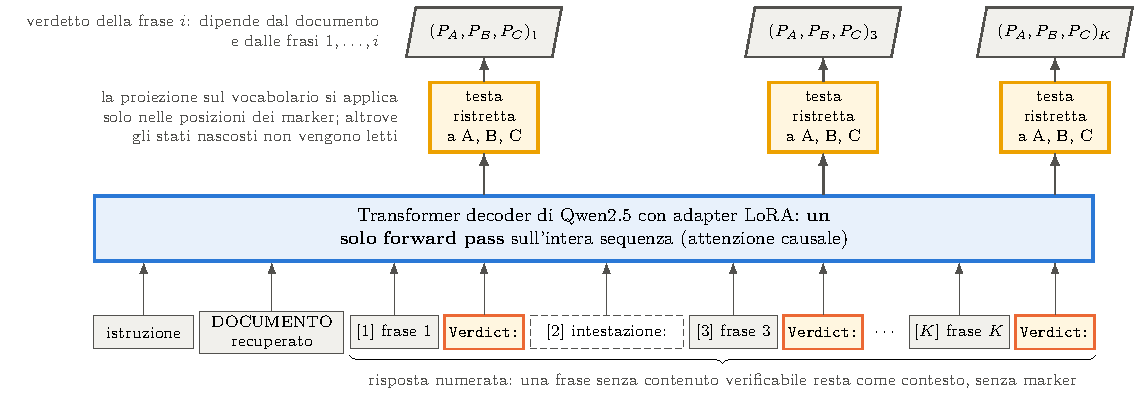
\includegraphics[width=0.86\textwidth]{../Thesis_ita/images/diagrams/method_marked_prompt_tikz.pdf}
\caption{Il prompt con i marker di GroundOne: i verdetti di tutte le frasi si leggono in corrispondenza dei marker
\texttt{Verdict:} in un solo forward pass.}
\label{fig:prompt}
\end{figure}

\sect{Dati e impostazione sperimentale}
Nessuna etichetta è stata annotata da capo: le annotazioni a span di RAGTruth sono state convertite in un'etichetta a tre
classi per frase con regole fissate in anticipo. Tre test set sono stati costruiti, verificati e congelati prima di
qualsiasi addestramento, con il leakage controllato a livello di documento: lo split di test di RAGTruth (nel dominio),
LLM-AggreFact (un benchmark ampio di groundedness) e VitaminC (un test di fact-checking fuori dominio). GroundOne è
confrontato con indizi che non leggono mai il documento, con i modelli non addestrati, con giudici LLM della stessa
dimensione con e senza probabilità, con due decision model generalisti (Rizzo-Flow e d1-3B di Liquid AI) e con encoder
specializzati (MiniCheck-RoBERTa, HHEM), tutti sulla stessa macchina e con intervalli di confidenza da un cluster
bootstrap.

\sect{Risultati}
La specializzazione funziona nel dominio a cui è rivolta. Su RAGTruth GroundOne è molto più accurato degli stessi modelli
prima dell'addestramento, ordina le frasi supportate meglio degli encoder specializzati e, in accuratezza a tre classi,
supera nettamente entrambi i decision model generalisti, compreso uno più grande. Su LLM-AggreFact il modello più grande è
alla pari con MiniCheck, non sopra. Su VitaminC il guadagno scompare e un decision model generalista è molto più forte: uno
specialista non è uno strumento generale di fact-checking. Il modo di leggere la decisione conta di per sé: con lo stesso
modello addestrato, scegliere tra le tre lettere ammesse è nettamente più accurato che lasciare al modello generare il
proprio verdetto, con la stessa latenza, e lo scarto è maggiore per il modello più piccolo.

GroundOne è più veloce dei giudici LLM della stessa dimensione a ogni lunghezza di risposta, e il vantaggio cresce con il
numero di frasi: sulle risposte lunghe è circa due volte più rapido di un giudice sintetico e più volte più rapido di uno
verboso, sempre con un output valido. Scomporre il tempo spiega perché il guadagno complessivo è moderato: la lettura di
documento e risposta è quasi tutto il tempo di GroundOne ed è comune a ogni approccio, mentre la parte di decisione, quella
che il readout sostituisce, costa oltre un ordine di grandezza meno della scrittura dei verdetti. Quando il documento è
già stato letto, come nella verifica di una risposta riscritta, il riuso della KV cache rende la verifica di GroundOne più
volte più rapida, ma aiuta molto meno i giudici, perché il loro decoding non si può riusare. GroundOne consuma anche meno
energia, anche se il risparmio è minore di quello sul tempo, perché un prefill lungo assorbe più potenza del decoding. Dopo
la calibrazione le sue probabilità sono vicine alle frequenze osservate, mentre i giudici LLM a cui si chiede lo stesso
output producono probabilità che distinguono appena le decisioni giuste da quelle sbagliate. La valutazione gira senza
rete e con risultati riproducibili, i pesi a 8 bit non costano accuratezza, e generatore e verificatore stanno insieme in
un unico processo con ampio margine di memoria.

\begin{table}[h]
\centering
\small
\begin{tabular}{>{\raggedright\arraybackslash}p{6.6cm}>{\raggedright\arraybackslash}p{8.4cm}}
\toprule
Domanda & Risultato \\
\midrule
Nel dominio (RAGTruth) & Forte guadagno sui modelli non addestrati; ordinamento migliore degli encoder; nettamente sopra entrambi i decision model generalisti. \\
Altri benchmark & Alla pari con MiniCheck su LLM-AggreFact; nessun guadagno su VitaminC, dove un generalista è più forte. \\
Readout e verdetto generato & Il readout ristretto è nettamente più accurato a parità di pesi e di costo. \\
Velocità rispetto ai giudici LLM & Più veloce a ogni lunghezza, soprattutto sulle risposte lunghe; molto di più con le fonti già in cache. \\
Probabilità & Ben calibrate dopo una semplice correzione post-hoc; quelle dei giudici quasi prive di informazione. \\
\bottomrule
\end{tabular}
\caption{Risultati principali in forma qualitativa; i valori esatti sono riportati nella tesi.}
\label{tab:results}
\end{table}

\sect{GroundOne Studio: un'applicazione locale e un caso di studio}
Un'applicazione nativa per macOS, scritta in Swift con MLX Swift, mette il verificatore al lavoro in un assistente RAG
completo in cui recupero (ricerca full-text di SQLite e un piccolo modello di embedding), generazione, verifica e un
giudice LLM locale condividono un unico processo, senza rete e ben dentro la memoria del portatile. Un test di conformità
mostra token identici e probabilità praticamente identiche a quelle dell'implementazione Python. La risposta del generatore
compare per prima; l'utente può poi verificarla con il solo GroundOne o insieme al giudice LLM, consultare le probabilità e
il passaggio a supporto di ogni frase e far riscrivere dalle fonti le frasi segnalate o selezionate, con una richiesta
breve per frase che dipende dal tipo di errore e un controllo che respinge una riscrittura identica alla frase segnalata.
In un caso di studio con errori iniettati GroundOne segnala quasi tutti gli errori, più spesso del giudice LLM, e la
riscrittura mirata ne rimuove la gran parte: numeri e date modificati vengono per lo più ripristinati dalla fonte, le frasi
inventate cancellate. Ripetere lo studio con il verificatore più piccolo mostra perché il verdetto a tre classi conta: il
modello etichetta i valori modificati come non menzionati anziché contraddetti, e il generatore li cancella invece di
correggerli. Un generatore più grande, selezionabile, corregge ancora più errori, ma è sensibilmente più lento e aggiunge
più contenuto che le fonti non riportano. Le risposte così ottenute sono accettate da GroundOne, non verificate in modo
indipendente.

\sect{Limiti e sviluppi futuri}
I limiti principali sono la ristrettezza dei dati di addestramento, a causa della quale le contraddizioni al di fuori del
data-to-text e le allucinazioni nascoste in frasi per il resto copiate vengono apprese solo in parte, una ricetta di
addestramento non del tutto robusta rispetto al seed, un'unica piattaforma e famiglia di modelli e dati soltanto in
inglese. Gli sviluppi futuri comprendono una ricetta più robusta (bias correction, gradient clipping, più seed), dati di
addestramento con supporto parafrasato e modifiche minime, la fusione dell'adapter nei pesi base, un porting su llama.cpp
per misurare altro hardware, adapter per lingua, l'attribuzione di ogni verdetto a un passaggio, la verifica durante la
generazione della risposta e un controllo indipendente delle frasi riscritte nell'applicazione.
\end{document}
